\documentclass[12pt,a4paper,openright,twoside]{book}
\usepackage[utf8]{inputenc}
\usepackage{amsmath}
\usepackage{amssymb}
\usepackage{listings}
\usepackage{algpseudocode}
\usepackage{tabularx}
\usepackage{graphics}
\usepackage{disi-thesis}
\usepackage{code-lstlistings}
\usepackage{notes}
\usepackage{shortcuts}
\usepackage{acronym}
\usepackage[linesnumbered,ruled,vlined]{algorithm2e}


\newcommand{\thesislang}{english} % commentare in caso di tesi in italiano
%\usepackage{thesis-style}
% version
%\newcommand{\versionmajor}{0}
%\newcommand{\versionminor}{1}
%\newcommand{\versionpatch}{2}
%\newcommand{\version}{\versionmajor.\versionminor.\versionpatch}
%\typeout{Document version: \version}

\school{\unibo}
\programme{Corso di Laurea Magistrale in Ingegneria e Scienze Informatiche}
\title{Fair-by-design algoriths for access to education}
\author{Antonio Iannotta}
\date{\today}
\subject{Intelligent Systems Engineering}
\supervisor{Prof. Giovanni Ciatto}
\cosupervisor{Prof. Roberta Calegari}
\morecosupervisor{Prof. Andrea Omicini}
\session{IV}
\academicyear{2022-2023}

% Definition of acronyms
\acrodef{IoT}{Internet of Thing}
\acrodef{vm}[VM]{Virtual Machine}
\acrodef{AI}{Artificial Intelligence}


\mainlinespacing{1.241} % line spacing in mainmatter, comment to default

\begin{document}
	
\frontmatter

% ! TeX root = thesis-main.tex
\title{Title}
\author{Candidate Name Here}
\date{\today}

\newgeometry{margin=0.8in}
\begin{titlepage}
	\begin{center}
		% \vspace*{0.2cm}
		
		\large
		\textbf{ALMA MATER STUDIORUM -- UNIVERSITÀ DI BOLOGNA \\ CAMPUS DI CESENA}
		\\
		\noindent\hrulefill
		\vspace{0.4cm}
		
		\Large
		Scuola di Ingegneria e Architettura \\
		Corso di Laurea Magistrale in Ingegneria e Scienze Informatiche
		
		\Huge
		\vspace{4cm}
		\textbf{
			Fair-by-design algorithm for access to education
		}
		
		\large
		\vspace{1cm}
		Tesi di laurea in 
		\\
		\textsc{Intelligent System Engineering}
		
		\vspace{5.5cm}
		\begin{minipage}[t]{0.64\textwidth}
			\begin{flushleft}
				\textit{Relatore} 
				\\ 
				\textbf{Prof.} \textbf{Giovanni Ciatto}
				\\
				\vspace{0.4cm}
				\textit{Correlatore} 
				\\
				\textbf{Prof.} \textbf{Roberta Calegari}
				\textbf{Prof.} \textbf{Andre Omicini}
			\end{flushleft}
		\end{minipage}
		\begin{minipage}[t]{0.34\textwidth}
			\begin{flushright}
				\textit{Candidato} 
				\\ 
				\textbf{Antonio Iannotta}
			\end{flushright}
		\end{minipage}\\
		
		\vfill
		\noindent\hrulefill
		\vspace{0.3cm}
		\Large
		
		IV Sessione di Laurea
		\\
		Anno Accademico 2022-2023
	\end{center}
\end{titlepage}
\restoregeometry


\begin{abstract}

    This work presents an in-depth approach to address fairness and bias mitigation in the design and development of data-driven methods. The primary contribution of this study is the proposal and implementation of an innovative \emph{Fair-by-Design} workflow that incorporates various strategies for bias mitigation within data, algorithms, and decision-making processes.

    The work focuses on the educational data of the Canary Islands, leveraging a dataset encompassing detailed information about student performance and educational outcomes.

    The primary objective is to ensure equitable and unbiased application of data-driven algorithms within the educational context. 

    The methodology involves the systematic evaluation of multiple bias mitigation strategies. The critical aspect of this research centers on the comparison of these strategies based on their impact on the predictive accuracy of the algorithms. 

    This approach provides practical insights into the trade-offs between fairness and accuracy, showing how several approaches can lead to different accuracy scores on the same dataset and with the same models. 

    The work findings offer valuable insights into the trade-offs between fairness and accuracy when developing data-driven methods for educational data. 

    This thesis contributes to the ongoing discourse on fairness in machine learning and data-driven decision-making. The results provide guidance for stakeholders in the education sector, aiding them in making informed decisions about algorithm deployment to promote fairness and minimize bias within educational systems. 

\end{abstract}
    


%\begin{acknowledgements} % this is optional
%Never too far down, to come back
%\end{acknowledgements}

%----------------------------------------------------------------------------------------
\tableofcontents   
%\listoffigures     % (optional) comment if empty
%\lstlistoflistings % (optional) comment if empty
%----------------------------------------------------------------------------------------

\mainmatter

%----------------------------------------------------------------------------------------
\chapter{Introduction}
\label{chap:introduction}
%----------------------------------------------------------------------------------------

Artificial Intelligence (AI) has experienced an unprecedented surge in prominence and utility in recent years, emerging as a transformative force across diverse domains. From powering autonomous vehicles to aiding healthcare diagnosis and recommendation systems, AI applications have become increasingly woven into the fabric of our daily lives. However, this rapid proliferation has ushered in a pressing concern about the pervasive presence of bias within AI systems.

The concept of bias in AI pertains to the inadvertent or systematic preference shown towards specific groups or characteristics within the data, algorithms, or decision-making processes. This partiality leads to outcomes that are unjust, unfair, and unequal. In this era of AI-driven decision-making, the imperative to address bias is not just a technological challenge but a moral and societal necessity. Additionally, the ethical principle of fairness underscores the collective aspiration to ensure that AI systems yield equitable and just results for all individuals, regardless of their personal attributes.

The repercussions of bias and unfairness in AI systems extend far beyond mere technological concerns. These issues carry profound societal implications, impacting vital areas such as employment, education, and access to critical services. Biased AI systems perpetuate and exacerbate existing inequalities, inadvertently reinforcing harmful stereotypes and undermining the foundational principles of justice and equality.

In the realm of education, data-driven decision-making has gained significant ground, with educational institutions increasingly relying on AI systems for tasks ranging from student admissions to evaluating learning outcomes and allocating educational resources. The stakes in this domain are notably high. Ensuring that these AI-driven education systems mitigate bias and prioritize fairness is not just a technological endeavor; it is a moral and societal imperative.

The Fair-by-Design workflow presented extends the traditional machine learning workflow by explicitly incorporating fairness considerations from the outset of AI system design. This approach aims to proactively address and mitigate bias throughout the development process, ensuring fairness is not an afterthought but an integral part of the system's foundation.

This work proposes the Fair-by-Design workflow, offering multiple solutions to address fairness challenges within AI systems. We explore and implement three distinct approaches within this workflow, each contributing to the overarching goal of fostering fairness in AI.

The objective is to compare not only the accuracy but also the value of specific fairness metrics at the conclusion of the workflow. By contrasting these outcomes with a scenario where fairness assumptions are not made, we aim to provide a comprehensive assessment of both accuracy and fairness within the proposed framework.

The structure of this thesis unfolds as follows: The \cref{chap:background} conducts a thorough review of the existing approaches and methodologies designed to address bias and promote fairness in the development of AI systems. This chapter lays the groundwork upon which our innovative Fair-by-Design workflow is built. The \cref{chap:contribution} chapter delves into the intricacies of the workflow, elucidating the seamless integration of various fairness approaches into the design process. The \cref{chap:validation} meticulously presents the results derived from the application of these fairness approaches, offering an empirical comparison of their performance and effectiveness. Finally, the \cref{chap:conclusions} not only imparts insights gleaned from our research but also outlines prospective directions for further advancements in this critical and ever-evolving field.

%----------------------------------------------------------------------------------------
\chapter{State of the Art} % or Background
\label{chap:background}

This chapter provides a comprehensive overview of the preceding works and the scientific literature that have paved the way for the implementation of fair-by-design methods in our research. The journey begins with a thorough examination of the multifaceted field of \textbf{artificial intelligence} and its wide-ranging applications, including its pivotal roles in critical sectors and socio-technical systems. Within this context, we delve deeply into the intricate issues of \emph{bias} and \emph{fairness} in AI systems, acknowledging the essential foundation upon which our work is built. 

Artificial Intelligence (\emph{AI}) stands at the forefront of technological innovation, significantly reshaping diverse sectors, from healthcare to finance and transportation. To comprehensively grasp the transformative potential of AI, it is essential to explore its applications and the complex ecosystems in which it operates. This chapter endeavors to unravel the intricate web of AI systems and their profound impact on society.

However, the proliferation of AI brings with it the inherent challenge of bias. As AI systems learn from vast datasets, they may inadvertently perpetuate and exacerbate existing prejudices, resulting in \textbf{bias} within the algorithms. Recognizing this challenge as a critical one, our exploration extends into the various dimensions of bias, highlighting its multifaceted nature and the potential consequences it carries. 

Moreover, in our quest for equitable AI, the concept of \emph{fairness} emerges as a beacon of hope. This chapter dissects the concept of fairness within AI systems, exploring the intricate ethical considerations that underlie the pursuit of equitable outcomes for all individuals. The chapter further investigates technical dimensions of fairness, acknowledging that it is not merely a goal but a fundamental ethical principle that underpins our work. 

Through this comprehensive exploration, we pave the way for the implementation of fair-by-design methods. This chapter is not only a testament to the foundation on which our research stands but also a testament to the complexity of the AI landscape, its potential for societal transformation, and the imperative of mitigating bias and promoting fairness as we forge ahead in the development of AI systems. 


\section{Artificial Intelligence}

This chapter embarks on a deep dive into the dynamic and multifaceted realm of Artificial Intelligence (AI) and Machine Learning (ML), two groundbreaking technologies that are reshaping human interaction with the world. AI, as a vast and encompassing domain, denotes the development of computer systems endowed with the capability to perform tasks traditionally reserved for human intelligence. These tasks span the spectrum from speech recognition to intricate problem-solving and adaptive learning. 

Within the expansive domain of AI, Machine Learning emerges as a prominent subset, taking center stage in this exploration. Machine Learning is a field that focuses on creating algorithms that empower computers to discern intricate patterns within data and make informed predictions. At its core, Machine Learning excels at enhancing performance over time by processing and assimilating data. The essence of Machine Learning lies in its ability to autonomously learn from data, continuously adapting and improving its decision-making capabilities. 

The AI and ML landscape encompasses a diverse array of techniques and methodologies. Notable examples include Natural Language Processing, Computer Vision, Robotics, and Expert Systems, each wielding distinct capabilities and applications. Machine Learning, in particular, is a repository of algorithms crafted to enable machines to self-learn and refine their performance sans explicit programming. These algorithms grant machines the ability to make data-driven decisions, essentially automating the process of pattern recognition and prediction. 

The transformative impact of AI extends far beyond the horizon, with direct implications for critical sectors, including healthcare and autonomous driving, where the consequences are not merely abstract but can be a matter of life and death. However, the profound influence of AI is not confined to these sectors alone. It permeates socio-technical systems, which are emblematic of the intricate interplay between individuals, technology, and social institutions. 

Socio-technical systems are marked by the intricate interplay between individuals, technology, and social institutions. AI and ML have catalyzed substantial transformations within these systems, profoundly altering how individuals interact with technology and reshaping the fabric of society. As AI becomes increasingly embedded in the social fabric, it is imperative to confront the intricate ethical quandaries it raises. 

The integration of AI and ML within these systems has precipitated a cascade of intricate ethical dilemmas. These encompass concerns surrounding data privacy, the pervasive presence of biases inherent in algorithms, and the impending potential for job displacement due to automation. In this context, constructing robust ethical frameworks is not just a matter of academic discourse but an essential imperative. 

These ethical frameworks serve as a safeguard, ensuring that AI systems adhere to the principles of fairness, transparency, and accountability. They stand as the bulwark against potential harm and serve to distribute the benefits of AI equitably across society. As this chapter unfolds, it endeavors to delve deeper into these ethical considerations, offering insights into how technology and ethics converge in the evolving landscape of AI and ML. \cite{GRUETZEMACHER2022102884}.

\newpage
\section{Traditional Machine Learning Workflow}

The traditional machine learning (ML) workflow comprises several fundamental steps, each playing a crucial role in the development of predictive models. These steps are designed to transform raw data into a trained and evaluated model. The following sections outline the four main stages of the traditional ML workflow: data acquisition, data pre-processing, modeling, and performance evaluation.

\subsection{Data Acquisition}

The first step in any machine learning project is acquiring the necessary data. This involves identifying and collecting datasets relevant to the problem at hand. The quality and quantity of the data directly impact the performance and generalization ability of the model. Data acquisition may involve obtaining datasets from public repositories, creating custom datasets, or integrating data from various sources.

\subsection{Data Pre-processing}

Once the data is collected, it undergoes pre-processing to make it suitable for training machine learning models. This stage involves cleaning the data to handle missing values, removing outliers, and addressing any inconsistencies. Additionally, feature engineering may be performed to extract relevant information and create new features. Data normalization or scaling may also be applied to ensure that all features contribute equally to the model.

\subsection{Modeling}

With pre-processed data, the next step is to select and train a machine learning model. This involves choosing an appropriate algorithm based on the nature of the problem (classification, regression, etc.) and the characteristics of the data. The selected model is then trained on a portion of the dataset, learning the patterns and relationships within the data. Hyperparameter tuning may be conducted to optimize the model's performance.

\subsection{Performance Evaluation}

The final stage of the traditional ML workflow is evaluating the model's performance on unseen data. This is typically done using a separate test dataset that the model has not encountered during training. Common evaluation metrics include accuracy, precision, recall, F1 score, and area under the receiver operating characteristic (ROC) curve. The goal is to assess how well the model generalizes to new, unseen instances and to identify areas for potential improvement.

\newpage
\section{Bias}

Artificial Intelligence (AI) is undeniably a transformative force, poised to reshape multiple dimensions of our existence in profound ways. Its versatile applications extend far and wide, from refining and expediting decision-making processes to seamlessly automating mundane and repetitive tasks. In this ever-evolving landscape, AI systems are becoming increasingly integrated into our daily experiences, orchestrating a paradigm shift in how we interact with the world around us. 

However, amidst the excitement and optimism surrounding AI's potential, a growing concern resonates both within the AI community and society as a whole. This concern revolves around the pervasive issue of biases intricately woven into the very fabric of AI algorithms. 

These biases, often unintentional and subtle, can seep into AI systems through the data they are trained on and the methods employed to develop them. As AI systems learn from historical data, they may inadvertently inherit the prejudices and stereotypes present in those datasets. Consequently, these biases can manifest in various ways, perpetuating and amplifying societal inequalities. For example, in AI applications for hiring or lending, biases can result in unfair discrimination based on factors such as race or gender. In automated content recommendations, biases can reinforce echo chambers, limiting exposure to diverse perspectives and ideas. 

The consequences of these biases are far-reaching and profound. They not only undermine the ethical foundations of AI but can also erode trust in these technologies. As AI systems gain prominence in critical areas like healthcare, criminal justice, and education, the ramifications of bias become increasingly worrisome. 

Addressing bias in AI is a complex and ongoing challenge. It requires a multifaceted approach that encompasses not only improved data collection and curation but also transparency in AI decision-making processes. Researchers and engineers are working tirelessly to develop techniques for bias detection and mitigation. Additionally, there is a growing push for diverse representation in the AI development community to ensure that the creation of AI systems considers a wide array of perspectives. 

In conclusion, while the promise of AI is immense, the journey towards harnessing its potential responsibly and equitably is an imperative one. As we move forward in this AI-driven era, it is essential to remain vigilant in identifying and rectifying biases, ensuring that AI truly serves as a force for positive change in our evolving world. \cite{10.1145/3308560.3317590}

\subsection{Understanding Bias in AI}

Bias in AI is a critical issue, signifying the presence of unjust and skewed representations or treatment of individuals or groups based on attributes such as race, gender, age, socioeconomic status, or other defining characteristics. These biases are deeply embedded in AI systems and can persist throughout their development and training processes. They arise from a variety of sources, including historical data imbalances, deeply ingrained societal prejudices, and imperfections in the algorithms themselves.

\subsection{Sources of Bias}

\subsubsection{Historical data} 

The issue of bias originating from historical data is a critical and intricate challenge that looms large in the landscape of machine learning. When machine learning models are trained on datasets culled from the annals of history, they inevitably inherit the biases and patterns encoded within that data. These historical biases, often a reflection of deeply ingrained societal prejudices and structural inequalities, can persist and intensify when the model is operationalized. \cite{10.1145/3308560.3317590}

Consider a scenario where historical data contains systemic biases against specific demographics, such as gender, race, or other socio-demographic attributes. The machine learning model, in its quest to optimize performance, dutifully replicates and perpetuates these biases in its predictions and decision-making processes. The consequence of this perpetuation is the perpetuation of historical injustices, potentially leading to the endorsement of discriminatory practices and the exacerbation of preexisting societal inequalities, significantly disadvantaging certain groups. 

Effectively addressing bias originating from historical data necessitates a multidimensional approach, coupled with proactive measures. The first step involves diligent data preprocessing techniques aimed at the identification and subsequent mitigation of bias-laden elements within the dataset. These techniques span a spectrum from data re-sampling to re-weighting and data augmentation, designed to restore balance and fairness. 

Simultaneously, interventions in algorithmic fairness are introduced to the machine learning process. These interventions encompass a range of techniques, including re-weighting of training instances, the introduction of fairness constraints, and adversarial debiasing methods, all aimed at guiding the model toward making fair and equitable predictions. 

Moreover, the journey toward equitable AI is an ongoing one, requiring constant vigilance. Continuous monitoring and adjustment of models, often in real-time, become imperative to ensure that fairness is upheld and biased outcomes are identified and rectified. 

Ultimately, the overarching goal is to foster a future where machine learning not only learns from historical data but actively works to transcend the bonds of bias. In this vision, AI systems operate as champions of fairness and social justice, contributing to the construction of a more equitable and just society where decisions and predictions are untainted by historical prejudices. This endeavor is not just a technical challenge but a moral imperative, driving the AI community to build a more equitable future for all.

\subsubsection{Human bias}

Bias introduced by human factors represents a pervasive and intricate challenge within the realm of machine learning. It is essential to understand that human bias, which can emanate from societal, cultural, or personal beliefs and attitudes, has the potential to inadvertently permeate the entire spectrum of the machine learning pipeline. This influence spans from the initial stages of data collection and annotation to the model training and decision-making processes. 

Human bias can manifest in multifarious ways, thereby complicating the quest for fair and unbiased machine learning models. These manifestations may include the biased selection of training data, subjectivity in annotations, or implicit prejudices that insidiously seep into the very fabric of algorithm design and evaluation. When humans are intricately involved in the decision-making processes or contribute to the development of algorithms, their biases, often unperceived, can become unintentionally embedded in the model. This results in a cascade of skewed predictions and the inadvertent reinforcement of preexisting societal inequalities. \cite{https://doi.org/10.1002/widm.1356} 

The recognition and mitigation of human bias represent an imperative for the development of equitable and just machine learning models. This mission encompasses several facets. First and foremost, it demands an elevated level of awareness within the machine learning community and society at large. Recognizing the potential pitfalls of human bias is a crucial step toward addressing them. 

Promoting diversity and inclusion, both in the workforce and in the datasets used for model training, is instrumental in countering human bias. Diverse perspectives and a multiplicity of experiences contribute to a more comprehensive and unbiased understanding of the world. 

Moreover, practical measures are implemented to detect and mitigate bias throughout the machine learning pipeline. This includes strategies ranging from fairness-aware machine learning algorithms to post-processing techniques that rectify biased predictions. 

The journey toward mitigating human bias is continuous and iterative. Machine learning practitioners continually refine their algorithms to minimize the impact of human bias and ensure that their models contribute to a more equitable and unbiased society. The ultimate goal is to harness the transformative potential of machine learning while eliminating the inadvertent perpetuation of human biases, thereby ushering in a more equitable and just era in technological advancement.

\subsubsection{Algorithmic bias}

Algorithmic bias, an intrinsic challenge in the domain of machine learning, underscores the presence of inherent biases that can manifest in the design, development, and deployment of machine learning algorithms. These biases, often unintended, can originate from a myriad of sources, encompassing factors such as biased training data, skewed feature selection, or implicit assumptions woven into the algorithm's development process. 

Algorithmic bias possesses the insidious potential to perpetuate and magnify preexisting societal prejudices and disparities, culminating in outcomes that are patently unfair and discriminatory. Consider the scenario in which a machine learning model is trained on historical data that inherently encapsulates societal biases. The model, in its endeavor to optimize predictive accuracy, inadvertently assimilates and reinforces these biases. The result is an algorithm that produces predictions and decisions that are tinged with bias, potentially aggravating societal inequalities and offering unequal treatment to specific groups. \cite{10.1145/2983270} 

Addressing algorithmic bias is a pivotal imperative when striving to construct equitable and just AI systems. This undertaking encompasses a comprehensive scrutiny of the entire machine learning pipeline, from data collection to model development and deployment. It commences with the meticulous assessment and rectification of bias within training data, aiming to restore balance and fairness. 

Furthermore, the integration of fairness-aware algorithms within the machine learning process is crucial. These algorithms are deliberately designed to recognize and rectify biases, offering a safeguard against discriminatory predictions and decisions. 

Transparency and fairness represent integral aspects of the decision-making process. The incorporation of these elements ensures that algorithms operate equitably, are devoid of bias, and actively promote fairness and equal treatment for all individuals, irrespective of their backgrounds. 

In essence, the mission of addressing algorithmic bias is pivotal for harnessing the true potential of AI systems. It involves forging a future where AI, far from perpetuating biases, serves as a champion of fairness and social justice, contributing to the construction of an equitable and just society in the digital age.


\subsection{Example of Bias in AI}

\subsubsection{Race and Gender Bias in Facial Recognition} 

Race and gender bias in facial recognition technology is a pressing and deeply concerning issue that underscores the ethical complexities tied to the development of AI. Facial recognition systems, often trained on large datasets, inadvertently perpetuate biases present in these datasets, particularly biases related to race and gender. The lack of diversity in training data, which is predominantly skewed towards certain demographics, results in algorithmic bias, where the system may struggle to accurately recognize individuals from underrepresented racial or gender groups. \cite{https://doi.org/10.5281/zenodo.4050457}

Studies have provided compelling evidence that these systems are often more accurate for individuals with lighter skin tones compared to those with darker skin tones, demonstrating a clear racial bias. Similarly, gender recognition algorithms may exhibit inaccuracies, especially for gender-nonconforming individuals, further exacerbating biases. 

The consequences of these biases are wide-ranging and profound. For instance, in law enforcement applications, the use of facial recognition may lead to the disproportionate targeting and misidentification of individuals from minority communities, potentially resulting in wrongful arrests and increased surveillance. In commercial contexts, biased facial recognition can significantly impact hiring processes, access to services, and overall societal fairness, with far-reaching implications for individuals and communities.


\subsubsection{Criminal Justice Bias}

Criminal justice bias is a deeply ingrained issue within the legal system that manifests through unequal treatment of individuals based on their race, socioeconomic status, gender, and other factors. The criminal justice system should ideally operate on principles of fairness, justice, and equality before the law. However, biases at various stages of the criminal justice process, from policing and arrest to trial and sentencing, often lead to discriminatory outcomes. \cite{doi:10.1080/10345329.2019.1658694} 

Racial bias is a significant concern, with people of color, especially Black individuals and communities, experiencing disproportionately higher rates of arrest, harsher sentencing, and a lack of trust in the system. Discriminatory practices such as racial profiling and racial disparities in sentencing contribute to this bias. Socioeconomic bias is another critical factor, where individuals from marginalized and low-income communities may face prejudice in the form of limited access to legal resources and unequal treatment within the legal process. \cite{9660177}  

Gender bias is prevalent, particularly against women and gender-diverse individuals. Women can face stereotypes and discriminatory attitudes that affect their treatment by law enforcement, the courts, and correctional facilities. Additionally, biases against LGBTQ+ individuals can result in unfair treatment and disparities in the criminal justice system. \cite{gebru2020race} 

Addressing criminal justice bias necessitates comprehensive reform. This includes implementing policies to combat racial and socioeconomic disparities, providing anti-bias training to law enforcement, encouraging diversity within the legal profession, and promoting transparency and accountability in the criminal justice process. Legislation, sentencing reform, community engagement, and the support of marginalized communities are also vital steps toward achieving a fair and impartial criminal justice system that upholds the principles of equity and justice for all.


\subsubsection{Recruitment Bias}

Recruitment bias is a critical issue within the hiring process, where unconscious or conscious prejudices and preconceived notions influence decision-making during candidate selection. It manifests in various forms, such as racial, gender, age, socio-economic, educational, or even appearance-based biases, and can significantly impact the composition of the workforce. \cite{mujtaba2019ethical} 

One of the most prevalent forms of recruitment bias is racial or ethnic bias. Hiring decisions can be influenced by stereotypes, leading to the underrepresentation of certain racial or ethnic groups in the workplace. Similarly, gender bias can result in disparities in hiring and promotion opportunities, favoring one gender over another. Age bias often affects older candidates who may be overlooked in favor of younger, perceived to be more 'tech-savvy' individuals. 

Educational and socio-economic biases can also seep into the hiring process, where candidates from prestigious institutions or privileged backgrounds may be given preferential treatment. Appearance-based biases, although highly unfortunate, can influence decisions, impacting individuals based on their physical attributes, such as weight, height, or even hairstyle. 

Addressing recruitment bias requires a multipronged approach. Firstly, raising awareness and providing training on unconscious bias is essential for hiring teams. Implementing structured and standardized interview processes, blind recruitment techniques (removing personally identifiable information), and diverse interview panels can help mitigate biases. Moreover, organizations should focus on promoting diversity and inclusion, fostering a culture that values different perspectives and backgrounds, and monitoring and analyzing recruitment data to identify patterns of bias. Striving for fairness and inclusivity in the hiring process not only leads to a more diverse workforce but also improves organizational innovation, creativity, and overall success.

\newpage
\section{Fairness} 

The pursuit of fairness within AI systems represents a dynamic and indispensable area of focus within the ever-expanding realm of artificial intelligence. At its core, fairness underscores an ethical and moral imperative to ensure that AI technologies and algorithms treat all individuals with equitable respect, devoid of bias or discrimination. As AI increasingly penetrates diverse facets of society, from decision-making processes to job recruitment, lending, and law enforcement, the salience of fairness is unequivocal. 

The pursuit of fairness in AI is an all-encompassing endeavor, entailing an array of considerations that orbit around the ambition to eliminate bias predicated on attributes such as race, gender, age, ethnicity, and socio-economic status. Bias in AI manifests in multifarious ways, originating from the training data's inherent biases or the algorithms themselves. Fair AI systems, therefore, endeavor to minimize these biases, upholding the principles of impartiality and justice in the outcomes they produce. 

In the quest for fairness, various fairness metrics and criteria have emerged, serving as quantifiable benchmarks for assessing the equity of AI systems. These include disparate impact, equal opportunity, and demographic parity. Disparate impact assesses the differential impact an AI system has on distinct demographic groups, while equal opportunity guarantees that the probability of a positive outcome remains consistent across all demographic segments. Demographic parity, on the other hand, centers on the proportional representation of various groups within AI-generated outcomes. 

Addressing fairness within AI systems necessitates the employment of an assortment of techniques. This involves pre-processing data to ameliorate biases, the modification of algorithms to instill them with fairness-awareness, and post-processing methods to ensure that outcomes are equitable. Furthermore, transparency and explainability are pivotal features of AI models, facilitating a deeper understanding of potential biases and nurturing trust in the technology. 

Emphasizing the ethical dimension, the pursuit of fairness in AI systems transcends the confines of technical solutions. It necessitates the active involvement of stakeholders, the incorporation of diverse perspectives, and a steadfast commitment to adhering to guidelines and regulations that prioritize fairness and impartiality. 

In essence, the journey to achieve fairness in AI systems is an ongoing and multifaceted odyssey, demanding relentless research, interdisciplinary collaboration, and unwavering ethical vigilance. The ultimate objective is the creation of AI technologies that steadfastly uphold the principles of fairness, contributing to a more inclusive, just, and equitable society. The continued pursuit of fairness in AI is not just a technical endeavor but a moral imperative, shaping the future of technology and its impact on society.

\subsection{Fairness Techniques in AI}

\subsubsection{Pre-processing}

Pre-processing focuses onThe pre-processing phase, an integral component of AI system development, is dedicated to the meticulous handling of data before it is utilized in the training of an AI model. This stage assumes paramount importance as it lays the foundation for equitable and unbiased AI systems, ensuring that the data used is both balanced and representative of the rich diversity inherent in the population. 

The objective of pre-processing is to rectify any imbalances, biases, or irregularities in the data, aiming to foster an environment where the AI model can operate without predisposition. The use of common pre-processing techniques is pivotal to this endeavor. These techniques encompass oversampling and undersampling, which seek to redress the imbalance in the distribution of data across various classes or groups. 

Additionally, pre-processing includes the meticulous removal of noise from the data. Noise, in this context, refers to extraneous or irrelevant information that could distort the model's learning process. The elimination of such noise serves to enhance the data's signal-to-noise ratio, improving the model's ability to discern meaningful patterns. 

Furthermore, the creation of balanced synthetic datasets is a valuable technique within the pre-processing repertoire. This involves the generation of new data points, often through the extrapolation of existing data, with the goal of augmenting the representation of underrepresented classes or groups. 

In summation, pre-processing is the cornerstone of equitable and unbiased AI system development. It encompasses a suite of techniques designed to foster balanced and representative data, enabling AI models to operate with impartiality and fairness, contributing to more equitable and unbiased outcomes. handling the initial data before it is used to train the AI model. This stage is crucial to ensure that the data is balanced and representative of the diversity in the population. Common pre-processing techniques include oversampling, undersampling, noise removal from the data, and creating balanced synthetic datasets.

\subsubsection{In-processing}

In-processing techniques represent a focused and interventionist approach that takes place directly during the model training phase. This method aims to instill fairness into the AI model at its core, ensuring equitable and unbiased outcomes. It is a precise and intricate strategy designed to mitigate bias and discrimination within the model's decision-making processes. 

One prominent in-processing technique involves the application of regularization methods. Regularization techniques are instrumental in penalizing the model when it demonstrates a discriminatory inclination, particularly with regard to certain sensitive features, such as gender or ethnic origin. By imposing penalties, the model is encouraged to refrain from exhibiting bias and to generate fair and impartial predictions. 

Another facet of in-processing techniques involves the alteration of cost functions. By modifying the cost functions, the model's training process is steered toward fairness. This modification ensures that the model pays a cost for making biased predictions, thereby incentivizing it to provide equitable treatment across different categories. 

In addition to regularization and cost function adjustments, in-processing techniques may encompass the manipulation of the model's predictions themselves. This manipulation can be guided by fairness constraints, ensuring that the model's outputs adhere to the principles of fairness and impartiality, especially concerning sensitive attributes. 

In summary, in-processing techniques serve as a focused and critical juncture in the quest for fairness within AI models. By intervening directly during the model training phase, these techniques work toward equitable and unbiased outcomes, promoting the development of AI technologies that contribute to a more just and inclusive society.

\subsubsection{Post-processing}

Post-processing, a crucial phase in the life cycle of AI models, unfolds after the model has been meticulously trained and has generated predictions. This phase assumes the role of a corrective and fine-tuning mechanism, primarily focusing on adjustments and modifications to the model's predictions with the overarching objective of ensuring fairness and equity. 

One key facet of post-processing involves the application of realignments or adjustments to the model's predictions. These realignments are designed to rectify any unjustified disparities among demographic groups, ensuring that the model's outcomes are equitable and devoid of bias. This process may entail recalibrations or other transformative actions applied to the model's results to mitigate any latent biases that may have emerged during the training process. 

The successful implementation of post-processing techniques hinges on a profound understanding of the specific fairness challenges inherent in both the data and the models. This demands a nuanced comprehension of the intricacies of the data, including potential sources of bias and discrimination. Furthermore, it requires a comprehensive grasp of the model's inner workings, discerning where and why biases may have arisen. 

Ongoing evaluation represents an indispensable element of the post-processing phase. Continual assessments and audits are essential to ensure that AI models adhere to ethical standards and actively promote fairness. This continuous vigilance and adjustment are pivotal in fostering AI technologies that contribute to the construction of a more equitable and just society. 

In essence, post-processing represents the culmination of efforts to instill fairness within AI models, serving as the final safeguard against bias and discrimination in the model's predictions.

\subsection{Pre-processing Techniques for Addressing Fairness in AI}

Pre-processing techniques in AI systems are a critical component of the machine learning pipeline, laying the foundation for robust and accurate model training. Pre-processing involves preparing and cleaning the raw data to ensure it is suitable for feeding into machine learning algorithms. This step is essential as the quality of input data significantly impacts the performance and effectiveness of the AI system. 

The pre-processing phase encompasses a variety of operations, including data cleaning, data transformation, feature selection, and feature engineering. Data cleaning involves handling missing or erroneous data, removing duplicates, and addressing inconsistencies. Data transformation includes normalization and scaling, ensuring that features are on a consistent scale to prevent biases in model training. Feature selection involves identifying and selecting the most relevant features for the model, reducing complexity and improving efficiency. Feature engineering involves creating new features or modifying existing ones to enhance the model's ability to capture patterns and make accurate predictions. 

Additionally, pre-processing techniques are crucial for handling imbalanced data, where one class significantly outnumbers the others. Techniques like oversampling, undersampling, or generating synthetic samples can help address this imbalance and improve model performance. Handling categorical data through techniques like one-hot encoding or label encoding is another vital pre-processing step to convert categorical variables into a format suitable for model training.

\subsubsection{Oversampling and Undersampling}

Oversampling and undersampling are techniques used to address class imbalance, where one class significantly outnumbers the others in a dataset. In the context of fairness, these techniques are employed to ensure that the AI model is not biased towards the majority class and that the predictions are fair and equitable for all classes, particularly when sensitive attributes like race, gender, or ethnicity are involved. \cite{9442706}

\begin{enumerate}

    \item \textbf{Oversampling}

    \begin{itemize}

        \item \textbf{Definition:} Oversampling involves increasing the number of instances in the minority class by generating synthetic samples or replicating existing ones.
        
        \item \textbf{Fairness Context:} Oversampling aims to boost the representation of underrepresented groups, promoting fairness and equal consideration of all groups. It prevents the model from exhibiting bias towards the majority group.
    
    \end{itemize}

    \item \textbf{Undersampling}

    \begin{itemize}

        \item \textbf{Definition:} Undersampling involves reducing the number of instances in the majority class by removing samples, ideally in a strategic and unbiased manner.
        
        \item \textbf{Fairness Context:} Undersampling can be employed to level the playing field by reducing the dominance of the majority group. This ensures that the model's predictions are not disproportionately influenced by the majority group, promoting fairness in the model's outcomes.
    
    \end{itemize}

\end{enumerate}

\subsubsection{Noise Removal}

Noise removal in the context of fairness typically refers to the process of identifying and mitigating the effects of noisy or incorrect data points that may introduce biases or distortions in the data used to train or evaluate machine learning models. In fairness considerations, noise removal plays a crucial role in ensuring that the AI system's predictions and decisions are as accurate and unbiased as possible, particularly when sensitive attributes like race, gender, or ethnicity are involved. \cite{NEURIPS2019_8d5e957f}

\subsubsection{Data Augmentation}

Data augmentation is a technique often used in machine learning and data preprocessing to artificially increase the size and diversity of a training dataset by generating new data points based on the existing ones. In the context of fairness, data augmentation can play a crucial role in addressing imbalances and biases in the data, particularly when sensitive attributes are involved. Here's how data augmentation can be applied in the context of fairness:

\begin{enumerate}

    \item \textbf{Generating Additional Data for Underrepresented Groups}
    
    \begin{itemize}

        \item In scenarios where certain groups or classes are underrepresented in the training data, data augmentation techniques can be used to create additional examples for those groups. \cite{sharma2020data}
    
    \end{itemize}
    
    \item \textbf{Balancing Class or Group Representation}
    
    \begin{itemize}
        
        \item Data augmentation can be employed to balance class or group representation in the training data. By creating synthetic data points for underrepresented groups, it helps ensure that the model is not biased towards majority groups.
    
    \end{itemize}
    
    \item \textbf{Feature Engineering for Fairness}
    
    \begin{itemize}
        
        \item Data augmentation can also involve feature engineering that considers sensitive attributes. For example, it can create new features that better capture the nuances and characteristics of underrepresented groups. \cite{10.14778/3461535.3463474}
    
    \end{itemize}
    
    \item \textbf{Fair Data Augmentation}
    
    \begin{itemize}
    
        \item In the fairness context, it's important to ensure that data augmentation techniques do not introduce additional biases. Care should be taken to create synthetic data that aligns with the fairness and equity goals of the AI system. \cite{10.1145/3531146.3534644}
    
    \end{itemize}

\end{enumerate}

\subsubsection{Bias Mitigation Algorithms}

Bias mitigation in the context of fairness refers to the process of identifying, reducing, or eliminating biases within machine learning models and algorithms, particularly those that could lead to unfair or discriminatory outcomes, often associated with sensitive attributes like race, gender, age, or ethnicity. The goal of bias mitigation is to ensure that AI systems provide equitable and unbiased predictions and decisions for all individuals or groups.

\subsubsection{Sensitive Attribute Removal or Neutralization}

In some cases, sensitive attributes (e.g., race, gender) can be removed from the dataset or transformed into more neutral representations. This prevents the model from relying on these attributes to make predictions, promoting fairness. \cite{NEURIPS2021_64ff7983}

These pre-processing techniques are essential steps in the AI development pipeline to ensure that the subsequent models are fair, unbiased, and capable of providing equitable outcomes across various demographic categories.

\subsection{In-processing Techniques for Addressing Fairness in AI}

In-processing techniques aim to mitigate fairness issues directly during the model training phase, influencing the learning process to ensure fairness in model predictions. These approaches target bias reduction and fairness promotion within the model's decision-making process. Several techniques can be employed during model training to achieve fairness:

\subsubsection{Regularization}

Regularization  aims to address and mitigate potential biases within models, particularly when sensitive attributes like race, gender, or ethnicity are involved. Regularization techniques work by adding constraints or penalties to the model's training process to reduce the impact of sensitive attributes on predictions and ensure that fairness is maintained. \cite{6137441}

\subsubsection{Reweighting Training Samples}

Reweighting training samples is a technique used to address bias and promote fairness in machine learning models, particularly when sensitive attributes are involved. This approach involves assigning different weights to training samples to influence the learning process of the model in a way that mitigates bias and ensures that predictions are more equitable. \cite{10.1145/3178876.3186133}

\subsubsection{Prejudice Remover Regularizer}

The Prejudice Remover Regularizer is a technique used to mitigate bias and promote equitable outcomes in machine learning models. It's a form of regularization that aims to reduce discrimination by encouraging the model to make predictions that are less influenced by sensitive attributes such as race, gender, or ethnicity. \cite{10.1007/978-3-642-33486-3_3}

\subsubsection{Demographic Parity Loss}

The Demographic Parity Loss is a fairness metric and regularization technique used to promote fairness and reduce bias, particularly with regard to sensitive attributes like race, gender, or ethnicity. It is designed to ensure that the predictions made by a model are distributed equally or fairly across different demographic groups. \cite{jiang2022generalized}

\subsubsection{Fair Adversarial Training}

Fair adversarial training is a technique used in the context of fairness to reduce bias and discrimination in machine learning models, particularly when sensitive attributes like race, gender, or ethnicity are involved. This approach incorporates adversarial networks into the training process to promote fairness and equitable outcomes. \cite{pmlr-v139-xu21b}

These in-processing techniques are vital tools in promoting fairness within AI models. Integrating them appropriately during model training can significantly contribute to reducing biases and achieving equitable outcomes across various demographic categories.

\subsection{Post-processing Techniques for Addressing Fairness in AI}

Post-processing techniques are applied after the model has been trained and predictions have been generated. Their purpose is to rectify any biases or disparities in the model's outputs and ensure fairness in the final outcomes. Several techniques can be employed during post-processing to promote fairness:

\subsubsection{Threshold Adjustments}

Threshold adjustment is a technique used to promote equity and reduce bias in machine learning models, especially in scenarios where sensitive attributes like race, gender, or age play a significant role. It involves modifying the decision threshold that determines whether a model's output is classified as a positive or negative prediction. This adjustment aims to balance the rates of false positives and false negatives across different demographic or group categories, ensuring that all groups are treated more fairly. \cite{10.1145/3447548.3467251}

\subsubsection{Additive Counterfactuals}

Additive counterfactual explanations in the context of fairness refer to a method used to assess and promote fairness in machine learning models. Counterfactual explanations are designed to provide insights into the impact of sensitive attributes on model predictions and help identify potential bias or discrimination. The "additive" aspect suggests that changes are made to the original input to create counterfactual scenarios, allowing for a better understanding of the fairness implications. \cite{NIPS2017_a486cd07}

\subsubsection{Equalized Odds Post-processing}

Equalized Odds Post-processing is a technique used to mitigate bias and promote equal treatment in machine learning models, particularly in scenarios involving binary classification tasks. This technique is applied after a model has made predictions and aims to adjust those predictions to ensure that equal error rates are achieved across different demographic or group categories. \cite{10.1145/3442188.3445902}

These post-processing techniques are crucial in rectifying biases and promoting fairness in AI models. Utilizing them effectively can lead to more equitable outcomes and decisions across various demographic categories.

\newpage
\section{Fair-by-Design}

Fair-by-design methods represent a proactive approach to addressing bias and promoting fairness in machine learning and artificial intelligence systems from their inception. These methods aim to embed fairness considerations into the design and development of algorithms and models to prevent bias from emerging in the first place. 

One key aspect of fair-by-design is the careful curation and preprocessing of training data to mitigate biases that might be present. For instance, techniques for re-sampling, re-weighting, and data augmentation can be employed to balance underrepresented groups in the data. 

Another critical element of fair-by-design methods involves the modification of algorithms to incorporate fairness-awareness. This can be achieved through the introduction of fairness constraints during the training process or through adversarial debiasing techniques. 

Furthermore, post-processing methods are often utilized to ensure that the outcomes of machine learning models are equitable. These methods can include adjusting the model's predictions to reduce disparities between different groups. 

The ultimate goal of fair-by-design methods is to create AI systems that, from their very conception, are inherently fair and unbiased. By considering fairness as a fundamental design principle, we can work towards eliminating discriminatory effects in AI systems, contributing to a more equitable and just technological landscape. 

\newpage
\section{Fairness metrics}

Fairness metrics play a crucial role in evaluating the performance of AI systems and ensuring equitable outcomes for diverse groups. These metrics provide quantitative measures to assess and mitigate bias within machine learning models. In this section, we will explore the general concept of fairness metrics and delve into three specific metrics: disparate impact, equalized odds, and demographic parity.

\subsection{General Overview}

Fairness metrics are quantitative tools designed to assess the impact of AI systems on different demographic groups. They help identify and address biases in model predictions, ensuring that the system does not disproportionately favor or disadvantage specific groups based on protected attributes such as race, gender, or age.

Common fairness metrics include disparate impact, equalized odds, demographic parity, and many others. These metrics are instrumental in evaluating the fairness and ethical implications of AI models, particularly in applications like hiring, lending, and education.

\subsection{Disparate Impact}

\textbf{Definition:}

Disparate impact measures the ratio of favorable outcomes for different demographic groups. It highlights situations where a particular group experiences a disproportionately adverse impact compared to others.

\textbf{Calculation:}
\[ DI = \frac{Pr(Y = 1|A=a)}{Pr(Y = 1|A=b)} \]

Where:
\begin{itemize}
    \item \( Y \) is the predicted outcome,
    \item \( A \) is the sensitive attribute (e.g., gender, race),
    \item \( a \) and \( b \) represent different values of the sensitive attribute.
\end{itemize}

\textbf{Interpretation:}

A disparate impact value close to 1 indicates fairness, while values significantly deviating from 1 suggest potential bias.

\subsection{Equalized Odds}

\textbf{Definition:}

Equalized odds ensures that the true positive rate and false positive rate are similar across different demographic groups. This metric focuses on achieving parity in both the benefits and errors of the model for different groups.

\textbf{Calculation:}

\[ \text{True Positive Rate (TPR)} = \frac{Pr(\hat{Y} = 1|Y = 1, A = a)}{Pr(Y = 1|A = a)} \]
\[ \text{False Positive Rate (FPR)} = \frac{Pr(\hat{Y} = 1|Y = 0, A = a)}{Pr(Y = 0|A = a)} \]

\textbf{Interpretation:}

Equalized odds is achieved when the TPR and FPR are approximately equal across all demographic groups.

\subsection{Demographic Parity}

\textbf{Definition:}

Demographic parity requires that the proportion of positive outcomes is the same for all demographic groups, regardless of the sensitive attribute.

\textbf{Calculation:}

\[ DP = Pr(\hat{Y} = 1|A = a) - Pr(\hat{Y} = 1|A = b) \]

\textbf{Interpretation:}

A value close to 0 indicates fairness, suggesting that the model's predictions are not influenced by the sensitive attribute.


In conclusion, fairness in AI is not just an ethical necessity but a fundamental requirement for fostering trust and ensuring the responsible and equitable deployment of AI systems. Moving into the evolving landscape of AI, the collective efforts must prioritize fairness to harness the true potential of AI for the greater good.
%Write background here.

%This section is likely to contain a lot of citations.
%
%For instance in \cite{AnzengruberSocInfo2013} the authors propose a novel means for tackling with the problem of preventing bad things from happening.

%----------------------------------------------------------------------------------------
\chapter{Contribution} % possible chapter for Projects
\label{chap:contribution}

\section{Introduction to the Fair-by-Design Workflow}

This chapter unveils the core of the research—an innovative Fair-by-Design workflow meticulously crafted to address the pressing issue of bias mitigation within AI systems. It is important to note that, among all the techniques presented in the \cref{chap:background}, this workflow primarily focuses on the concepts of pre-processing techniques for bias mitigation. 

The Fair-by-Design concept underlines the commitment to infusing fairness principles into the very fabric of AI development. It signifies the endeavor to create AI systems that are not only technologically proficient but also ethically responsible. 

The Fair-by-Design workflow serves as the linchpin of this research. It guides the approach to designing and developing AI systems that are inherently fair, impartial, and equitable. The challenge of bias mitigation cannot be relegated to a mere post hoc consideration; it must be foundational. By introducing fairness considerations at the outset of the AI system design, the aim is to rectify biases before they become ingrained in decision-making processes. 

In the pages that follow, the intricacies of this workflow will be explored, providing a step-by-step elucidation of its various components and how they collectively contribute to the realization of a fair and unbiased AI system. This workflow will not only be a central theme throughout this chapter but also a thread that ties the entire thesis together. It signifies the commitment to addressing bias and promoting fairness within AI systems, particularly in the context of the educational domain. 

The journey will embark on a comprehensive exploration of the Fair-by-Design workflow, with the ultimate goal of mitigating bias, ensuring fairness, and achieving equitable outcomes in AI-driven decision-making.

\section{Workflow description}

The Fair-by-Design workflow is structured upon the conventional machine learning (ML) workflow, with notable modifications in data acquisition, data pre-processing, and performance evaluation. The modeling stage adheres to traditional ML practices, focusing on algorithm selection and training.

This section delves into the specifics of these adaptations, illustrating how the Fair-by-Design workflow introduces a nuanced approach to data acquisition, redefines data pre-processing strategies, and enhances the performance evaluation process. By retaining the robust modeling methodologies of traditional ML, the Fair-by-Design workflow integrates established techniques with a heightened commitment to fairness, ensuring equitable outcomes in machine learning applications.

\subsection{Data Acquisition}

In the Fair-by-Design workflow, the data acquisition process extends beyond the traditional scope by placing a heightened emphasis on the intricacies of the data, particularly underscoring the identification and understanding of sensitive attributes. While conventional data acquisition primarily concentrates on the collection of relevant datasets, the Fair-by-Design approach recognizes the imperative of delving into sensitive attributes, which proves pivotal in the evaluation of fairness.

The importance of understanding these sensitive attributes cannot be overstated, as they wield substantial influence over the fairness of the model's outcomes. This understanding is multifaceted, encompassing various dimensions such as legal considerations, ethical implications, and societal norms. Obtaining this knowledge is a nuanced process that often involves direct communication with stakeholders. In certain scenarios, sensitive attributes may be deliberate business choices, and engaging with stakeholders becomes crucial to discern the underlying motivations and expectations.

Alternatively, common-sense reasoning is applied to identify potential sensitive attributes that might impact fairness. This involves a thoughtful and context-specific analysis of the data, taking into account historical and societal contexts. Common-sense reasoning acts as a supplementary approach, especially in cases where direct communication might be limited or where latent, non-obvious sensitive attributes could influence the model's outcomes.

Once the data has been acquired, and a comprehensive understanding of sensitive attributes has been obtained, the Fair-by-Design workflow progresses to the next crucial step: fairness evaluation. This stage is fundamental as it sets the foundation for subsequent model development. The fairness evaluation is designed to rigorously assess the fairness of the dataset concerning the identified sensitive attributes. This involves quantitative analysis, statistical testing, and the application of fairness metrics, ensuring a systematic and objective evaluation of potential biases and disparities within the dataset.

By incorporating this nuanced and comprehensive approach to data acquisition and fairness evaluation, the Fair-by-Design workflow establishes a robust foundation for the development of machine learning models that not only meet technical performance criteria but also adhere to ethical and fairness considerations. The insights gained from this initial phase guide the subsequent stages of the workflow, contributing to the overall integrity and equity of the machine learning process.

\subsubsection{Fairness Assessment}

The fairness assessment within the Fair-by-Design workflow represents a critical checkpoint, functioning as a meticulous examination to ascertain the absence of biases and the alignment of the dataset with ethical considerations. At this stage, the objective is to rigorously evaluate the fairness of the dataset, particularly in relation to the identified sensitive attributes. This process is pivotal in establishing the ethical foundation of the subsequent stages in the machine learning pipeline.

To conduct this comprehensive evaluation, the Fair-by-Design workflow leverages Disparate Impact, a widely recognized and utilized fairness metric. Disparate Impact offers a quantitative measure of the differential treatment experienced by distinct groups within the dataset. Specifically, it assesses the ratio of favorable outcomes for various demographic groups, shedding light on potential biases and disparities that might be present.

The implementation of Disparate Impact serves as a vital indicator during the data acquisition phase, allowing practitioners to make well-informed decisions pertaining to fairness considerations. By quantifying the differential impact on different demographic groups, Disparate Impact facilitates a nuanced understanding of potential imbalances within the dataset, empowering practitioners to address and rectify biases before proceeding with subsequent stages of the machine learning pipeline.

The strategic integration of Disparate Impact into the fairness assessment phase underscores the commitment of the Fair-by-Design workflow to a principled and thorough approach in ensuring fairness. This metric acts as a guiding compass, steering practitioners towards fair and equitable machine learning practices from the outset of the workflow.

\subsection{Data pre-processing}

The data pre-processing step in the Fair-by-Design workflow is designed as a comprehensive process, integrating both traditional and fairness-oriented sub-steps. The workflow envisions two primary sub-steps to ensure the dataset's readiness for subsequent model development.

\subsubsection{Usual Pre-processing Step}

The first sub-step in data pre-processing addresses typical operations aimed at enhancing the overall quality of the dataset. Handling missing values is a crucial pre-processing task. In this workflow, NaN values are filled using the mean for continuous attributes and the median for discrete attributes. This conventional operation ensures a more complete and standardized dataset.

However, the Fair-by-Design workflow goes beyond standard pre-processing by incorporating operations specific to protected attributes and the output variable. These operations set the stage for defining the learning prediction goal and establishing how the protected attributes should be treated.

\begin{itemize}
    
    \item \textbf{Handling Protected Attributes:} 
    
    Within the Fair-by-Design workflow, an intricate transformation process is applied to protected attributes, which are assumed to be categorical in nature. This transformative step is crucial for ensuring fairness in the subsequent stages of the machine learning pipeline. The goal is to mitigate potential biases associated with these protected attributes and to create a representation that fosters equitable treatment within the model.

    The process begins by identifying the most frequent value for each categorical protected attribute in the dataset. This meticulous calculation ensures a comprehensive understanding of the prevalent categories within these attributes. Subsequently, a binary encoding scheme is employed to represent the protected attributes in a format conducive to machine learning model interpretation.

    In this encoding scheme, instances in the dataset where the protected attribute assumes the most frequent value are replaced with the binary representation 1, signifying a state of privilege concerning that specific attribute. Conversely, all other instances where the protected attribute takes on values different from the most frequent one are replaced with the binary representation 0. This binary encoding not only simplifies the representation of protected attributes but also facilitates the model's ability to distinguish instances based on their privilege or lack thereof concerning specific attributes.

    This nuanced encoding strategy is instrumental in transforming categorical protected attributes into a format that aligns with the fairness objectives of the Fair-by-Design workflow. The binary representation not only preserves the essential information about the protected attributes but also ensures that the subsequent machine learning model can effectively incorporate and act upon this information during training and prediction phases.

    By employing this detailed transformation process, the Fair-by-Design workflow establishes a foundation for unbiased and fair treatment of instances within the model. This step is integral to addressing potential disparities associated with protected attributes, ultimately contributing to the development of a more equitable and ethically sound machine learning model.
    
    \item \textbf{Handling Output Variable:} 
    
    The handling of the output variable in the Fair-by-Design workflow is a nuanced process that adapts to the nature of the variable, whether categorical or continuous. This tailored treatment is essential for aligning the prediction task with the fairness objectives of the workflow, ensuring that the model's predictions are not only accurate but also ethically sound.

    In cases where the output variable is categorical, the workflow initiates by determining the most frequent value within this category. This strategic calculation provides insights into the prevailing outcome within the dataset. Subsequently, instances where the output variable matches this most frequent value are replaced with the binary representation 1, while all other instances take on the binary representation 0. This transformation effectively redefines the prediction task, shifting the focus to discerning whether a given sample belongs to the most frequent outcome. This binary encoding approach not only simplifies the representation of categorical outcomes but also enables the model to make predictions in a manner that aligns with fairness considerations.

    Conversely, when the output variable is continuous, the workflow employs a distinct strategy. Values of the continuous variable that surpass the mean are replaced with 1, while those falling below the mean assume the binary representation 0. This adjustment transforms the prediction task into establishing whether a sample's continuous output is above the mean. This approach ensures that the model is not only attentive to the central tendency of the continuous variable but also considers the distribution of values concerning the mean. By adopting this methodology, the Fair-by-Design workflow addresses potential biases associated with continuous outcomes, promoting fairness and transparency in the prediction process.

    This tailored and meticulous treatment of the output variable underscores the commitment of the Fair-by-Design workflow to equitable and ethical machine learning practices. The workflow not only adapts to the inherent characteristics of the data but also ensures that the subsequent model operates with a heightened awareness of fairness considerations, contributing to the development of a more responsible and unbiased machine learning model.

\end{itemize}

This nuanced pre-processing step sets the groundwork for a fair and unbiased learning prediction, aligning the dataset with the ethical considerations embedded in the Fair-by-Design workflow.

\subsubsection{Fairness pre-processing algorithms}

The second sub-step of the data pre-processing phase in the Fair-by-Design workflow is meticulously crafted to address and mitigate bias in the dataset, employing a pre-processing approach explicitly designed for fairness considerations. This phase builds upon the dataset and protected attributes obtained during the data acquisition phase, introducing three distinct algorithms strategically devised to promote fairness.

The proposed algorithms are elucidated as follows:

\begin{itemize}

    \item \emph{Fairness through Unawareness with Proxy Detection via Association Rules Mining:} This algorithm harnesses the principles of association rule mining to detect proxies within the dataset. Proxies, in this context, refer to factors that may act as intermediaries, influencing the model's predictions and potentially leading to biased outcomes. By identifying and mitigating the impact of both protected attributes and potential proxies, this algorithm aims to enhance fairness in the dataset. Detailed insights into the design, implementation, and specific fairness considerations addressed by this algorithm will be expounded upon in \cref{section:fairness}.
    
    \item \emph{Fairness through Unawareness with Proxy Detection via Variables Only:} Similar to the aforementioned approach, this algorithm focuses on averting the impact of protected attributes. However, it places specific emphasis on considering only the protected attributes during the proxy detection process. The distinctions between this approach and the association rules mining-based approach will be thoroughly delineated in \cref{section:fairness}.
    
    \item \emph{Fairness through Data Rebalancing:} In a departure from the first two approaches, which aim to mitigate the effects of specific attributes, this algorithm adopts a data rebalancing strategy. The primary goal is to render the dataset fair by proposing a novel fairness definition and redistributing the data distribution. This approach introduces a new dimension to fairness considerations, focusing on rebalancing the dataset to mitigate biases and ensure equitable representation. The intricacies of the design, implementation, and the novel fairness perspective proposed by this algorithm will be dissected in \cref{section:fairness}.

\end{itemize}

The forthcoming section (\cref{section:fairness}) will provide an in-depth exploration of each algorithm, offering a comprehensive understanding of their theoretical underpinnings, practical implementation, and the specific fairness considerations they target. This detailed examination aims to equip practitioners with the insights necessary to make informed decisions about algorithm selection within the Fair-by-Design workflow.

\subsection{Performance evaluation}

After the model has undergone the training process, the evaluation phase in the Fair-by-Design workflow extends beyond traditional accuracy-based assessments. This phase places particular emphasis on incorporating fairness metrics to comprehensively evaluate the model's performance and rigorously assess the fairness of the entire workflow.

In the realm of fairness assessment, two key metrics, namely \emph{Equalized Odds} and \emph{Demographic Parity}, play a pivotal role in quantifying and analyzing the fairness implications of the model's predictions:

\begin{itemize}

    \item \emph{Equalized Odds:} This metric is designed to ensure parity in the true positive rate and false positive rate across different demographic groups. Mathematically, it involves minimizing the disparities in error rates between various subgroups. By focusing on achieving equity in both the benefits (true positives) and errors (false positives) of the model for diverse demographic groups, Equalized Odds offers a nuanced perspective on fairness. It provides a more granular understanding of how the model performs across different segments of the population, allowing practitioners to identify and rectify potential biases in prediction outcomes.
    
    \item \emph{Demographic Parity:} Demographic Parity is a fundamental fairness metric that mandates the proportion of positive outcomes to be the same for all demographic groups, irrespective of the protected attributes. This metric serves as a cornerstone for evaluating the overall fairness in the distribution of positive outcomes. It ensures that the model does not disproportionately favor or disadvantage specific demographic groups, contributing to a more unbiased and equitable evaluation of the model's performance. Demographic Parity provides valuable insights into the distributional aspects of the model's predictions and aids in uncovering any systemic disparities in positive outcome rates among different subgroups.

\end{itemize}
The integration of these advanced fairness metrics in the evaluation process enhances the transparency and ethical considerations of the Fair-by-Design workflow. Beyond traditional accuracy metrics, these fairness metrics offer a more nuanced understanding of how the model impacts different demographic groups, promoting a comprehensive evaluation of fairness implications. The upcoming sections will delve into a detailed analysis of the results obtained through the application of these metrics, providing deeper insights into the fairness considerations of the developed machine learning model.

Here's the graphical representation of the presented workflow:

\begin{center}

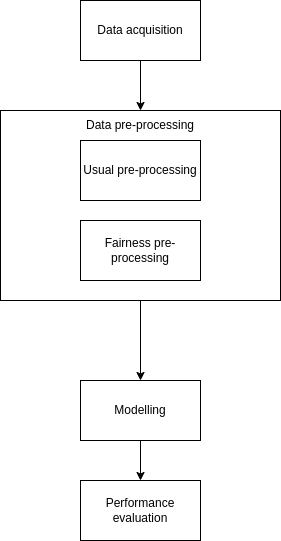
\includegraphics[width=.5\textwidth, height=1.0\textwidth]{fairness-workflow.png}

\end{center}

\newpage
\section{Fairness pre-processing algorithms}
\label{section:fairness}

The pivotal junction of the Fair-by-Design workflow lies in the meticulous design of fairness pre-processing algorithms. In this section, we delve into the intricacies of the algorithms and illuminate the thought process that guided their creation. These algorithms are not mere standalone entities; they are intricately woven into the fabric of the Fair-by-Design workflow, drawing inspiration and guidance from the overarching principles that define this ethical machine learning approach.

Each algorithm detailed in this section is a product of deliberate design choices, carefully tailored to address specific fairness considerations within the context of the workflow. We unravel the decisions underpinning the algorithms, exposing the rationale behind their unique structures. The transparency and interpretability of these design choices aim to empower practitioners with a deep understanding of how fairness is embedded into every layer of the pre-processing phase.

Moreover, the algorithms showcased here are not developed in isolation. Instead, they are fully influenced by the broader Fair-by-Design workflow they inhabit. This symbiotic relationship ensures that the algorithms seamlessly align with the workflow's core principles and ethical imperatives. Every line of code, every parameter choice, and every decision made in these algorithms bears the indelible mark of the fairness-centric philosophy that propels the Fair-by-Design methodology.

As we navigate through the nuances of each fairness pre-processing algorithm, the synthesis of design choices and workflow integration will become apparent. This section serves as a testament to the conscientious development of algorithms that not only rectify biases but do so in harmony with the overarching goal of fostering fairness and equity in the machine learning landscape. Join us on this exploration as we unravel the intricacies of algorithms shaped by design, ethics, and the guiding principles of the Fair-by-Design framework.

\subsection{Fairness through unawareness with proxy detection}

TThe algorithm elucidated in this section seamlessly integrates with the Fair-by-Design workflow, embodying the core concept of \emph{fairness through unawareness}. Rooted in the overarching goal of mitigating bias, this approach represents a significant stride in addressing fairness considerations within the machine learning pipeline.

The design choices of this algorithm are inherently influenced by the protected attributes detected during the data acquisition step of the Fair-by-Design workflow. Recognizing that bias may emanate not only from explicit protected attributes but also from indirect influences, the algorithm extends its reach beyond the conventional scope.

In alignment with the Fair-by-Design ethos, this algorithm advocates for the removal of both identified protected attributes and a set of strategically identified proxy variables. These proxy variables, akin to shadows of potential bias, are meticulously pinpointed and eliminated. The vigilance in detecting these proxies is inspired by the commitment to unravel and rectify any factors that might indirectly contribute to bias within the AI system.

Drawing insights from the comprehensive analysis conducted during the data acquisition phase, the algorithm takes a holistic view of potential sources of bias. The removal of proxy variables, guided by this understanding, exemplifies a proactive stance in addressing bias from multiple dimensions.

Citing Gupta et al.'s work on proxy variables in AI systems \cite{Gupta2018ProxyF}, the algorithm's incorporation of this innovative element underscores a commitment to not only meet accuracy standards but also to foster equity and fairness. The dynamic interplay between the algorithm's design choices and the Fair-by-Design workflow amplifies its effectiveness in creating AI systems that are not only precise but also inherently just, unbiased, and equitable.

In essence, this algorithm serves as a testament to the continuous evolution and refinement within the Fair-by-Design framework, where each step is meticulously crafted to reinforce the principles of fairness and transparency.

At this point it's necessary to begin with a formalization for the algorithm itself. It's important to consider that there are two versions of this algorithm: a version in which the proxy detection is performed exploiting the concepts embedded into the association rule mining theories, more specifically using the \emph{fp-growth} algorithm. In the other version the proxy attributes are inferenced from the variables only.

Let's consider a dataset \( D \) belonging to \( \mathbb{R}^{n \times m} \) with \( k \) protected variables.

\textit{fairness\_evaluation} is defined as follows:
\[
\text{fairness\_evaluation}(v_i, Y) = \lambda(v_i, Y) \quad \forall i \in [1, k]
\]

where:
\begin{align*}
v\_i & : \text{ith attribute belonging to the protected variables}, Y & : \text{output column}.
\end{align*}

The fairness metric \( \lambda \) evaluates the relationship between a protected attribute \( v_i \) and the output \( Y \), producing a value that represents the level of fairness for that protected attribute. It's important to consider that the output used for the fairness metric is not strictly related to the output of the dataset but, as showed further in this section it may also be a protected attribute. This lead to the consideration that protected attributes and output variable, that are the inputs of the fairness metric, are dependent on the specific scenario in which the fairness metric is applied.

\textit{dataset\_fair} is defined as follows: a dataset \( D \) is considered fair if for every value \( v \) belonging to \textit{fairness\_evaluation}, the following condition holds:
\[ 0.8  < v < 1.25 \] 

\subsubsection{Proxy detection via attributes only}

Let's consider the set \( A \), represented as the set of all variables in the dataset excluding the protected variables, and the set \( B \), representing the protected variables.

\textit{proxy\_detection} is defined as follows: for every variable \( \text{var} \) belonging to \( A \) and for every protected variable \( \text{var\_protected} \) belonging to \( B \), the variable is a proxy if the fairness metric \( \lambda(\text{var}, \text{var\_protected}) \) satisfies the condition:

\[
\lambda(\text{var}, \text{var\_protected}) <= 0.8 \quad \text{or} \quad \lambda(\text{var}, \text{var\_protected}) => 1.25
\]

In other words, a variable \( \text{var} \) is considered a proxy if the fairness measure \( \lambda \) between \( \text{var} \) and a protected variable \( \text{var\_protected} \) falls outside the acceptable range ]0.8, 1.25[.

\subsubsection{Proxy detection via fp-growth algorithm}

It's important to give a brief background of the Association Rule Mining, the family algorithm \emph{fp-growth} belongs to.

\begin{enumerate}
    
    \item \emph{Association rule mining}:

        Association rule mining represents a pivotal data mining technique employed to unearth intriguing relationships and patterns hidden within extensive datasets. This technique is specifically tailored to the task of identifying associations and correlations among diverse elements present in the data, thereby revealing valuable insights and connections that might otherwise remain concealed. 

        The primary objective of association rule mining is to expose the inherent dependencies between data items or attributes. It scrutinizes the dataset in search of rules that reveal the co-occurrence and relationships between different items. These rules often manifest in the form of "if-then" statements, where the presence of one item is associated with the presence or absence of another. 

        This technique is particularly advantageous when applied to large volumes of data, as it excels in discovering subtle, non-obvious associations that might elude simple statistical analysis. Association rule mining is a versatile tool with a wide array of applications, spanning domains such as market basket analysis, recommendation systems, and fraud detection. 

        The process of association rule mining involves the generation of itemsets and the identification of frequent itemsets—combinations of items that appear together frequently. The algorithm then extracts association rules from these frequent itemsets, offering valuable insights into the relationships and co-occurrences within the data. 

        The outcomes of association rule mining have the potential to drive informed decision-making, such as product recommendations based on customer purchase history, optimizing supply chain management, and identifying suspicious patterns in financial transactions.

    \item \emph{Fp-growth}:
    
        The FP-Growth (Frequent Pattern Growth) algorithm is a popular and efficient method for mining frequent itemsets in a transaction database. It is particularly used in association rule mining, where the goal is to discover interesting relationships between variables in large datasets.

        Here's a deeper explaination on this algorithm:

        \begin{itemize}

            \item \emph{Frequent Itemsets}: An itemset is a collection of one or more items in a transaction, while a frequent itemset is one that appears in a dataset with a frequency greater than or equal to a specified minimum support threshold.
            
            \item \emph{The FP-Growth Process}: The FP-Growth algorithm employs a divide-and-conquer strategy to mine frequent itemsets efficiently. It constructs a data structure called the FP-tree (Frequent Pattern tree) from the given dataset.
            
            \item \emph{Building the FP-Tree}: The dataset is initially scanned to determine the frequency of each item. Items are sorted in descending order of frequency, and the dataset is reprocessed to build the FP-tree. The FP-tree is a compact representation of the dataset, where each path from the root to a leaf represents a frequent itemset.

            \item \emph{Mining Frequent Itemsets}: Frequent itemsets can be extracted directly from the FP-tree without the need for repeated database scans. The algorithm recursively mines the FP-tree, considering conditional databases for each frequent item in the tree.

            \item \emph{Association Rule Generation}: Once frequent itemsets are identified, association rules can be generated. These rules express relationships between items based on their co-occurrence in transactions.

        \end{itemize}

        Let's define some terms:

        \begin{itemize}

            \item \emph{Itemset}: $I = \{i_1, i_2, \ldots, i_k\}$, where $i$ represents an item.

            \item \emph{Transaction Database}: $D = \{T_1, T_2, \ldots, T_n\}$, where $T$ is a transaction.

        \end{itemize}

        At this point it's important to introduce some mathematical notation

        \begin{itemize}

            \item \emph{Support Count ($\text{supp}(I)$)}: The number of transactions in the database containing the itemset $I$. $\text{supp}(I) = |\{T \in D : I \subseteq T\}|$ 

            \item \emph{Support ($\text{supp}(I)$)}: The fraction of transactions in the database that contain the itemset $I$. $\text{supp}(I) = \frac{\text{supp}(I)}{|D|}$

            \item \emph{FP-Tree}: The FP-tree is a tree structure where each node represents an item, and the paths from the root to the leaves represent frequent itemsets.

            \item \emph{Conditional FP-Tree}: For a given item $i$, the conditional FP-tree is constructed from the database by considering only transactions containing $i$.

        \end{itemize}

\end{enumerate}

After having introduced the necessary theoretical concepts here's presented the approach to detect the proxy attributes for the protected attributes previously established.

\textit{proxy\_detection} is defined as follows: for each antecedent \( A_i \) belonging to the antecedent list \( \mathcal{A} \), for each consequent \( C_j \) belonging to the consequent list \( \mathcal{C} \), and for each protected variable \( V_k \) belonging to the protected variable list \( \mathcal{V} \), \( A_i \) is a proxy if the fairness metric \( \lambda(A_i, C_j) \) is such that:

\[\lambda(A_i, C_j) <= 0.8 \quad \text{or} \quad \lambda(A_i, C_j) >= 1.25\]

In other words, an antecedent \( A_i \) is considered a proxy if the fairness measure \( \lambda \) between \( A_i \) and a consequent \( C_j \) is outside the acceptable range ]0.8, 1.25[.

Here it's possible to notice how, as previously said, the concepts of protected attributes and output provided as inputs for the fairness metric are dependent on the scenario. While the typical scenario involves the protected attribute as input together with the output of the dataset, in this one the protected attribute acts like the output while the actual protected attributes are inferred from the results of the metric.

There are two other fucnctions that needs to be defined in order to complete the algorithm.

%%% NECESSARY TO CHANGE THE FUNCTIONS TO RETURN THE VARIABLES TO RETURN TE PROXY AND PROTECTED ATTRIBUTES

\subsubsection{Pseudocode}

In the following is presented the pseudocode for the algorithm, in its two different versions, presented above.

%----------------------------------------------------------------------------------------
\chapter{Validation} % possible chapter for Projects
\label{chap:validation}
%----------------------------------------------------------------------------------------
Following the information reported into the \emph{Dataset} section the models presented in the following have been trained with the goal to predict wether the english level is above or behind the thershold. 

For each grade have been applied the following approaches, in order to perform a proper comparaison:
\begin{enumerate}
    \item No fairness assumptions are made
    \item Fairness through unawareness
    \item Fairness through unawareness with proxy detection via apriori
    \item Fairness through unawareness with proxy detection via variables only
    \item Fairness through data rebalancing
\end{enumerate}

\section{Experiment setup}
For each of the previous approaches have been chosen 3 models to perform the prediction:
\begin{enumerate}
    \item \text{RandomForest Classifier}: RandomForest Classifier is a popular machine learning algorithm that leverages an ensemble of decision trees to make predictions. It excels at tasks like classification and regression, offering robustness against overfitting and high accuracy by aggregating the predictions of multiple decision trees. It's a versatile tool used in various applications, from finance to healthcare and image analysis.
    \item \textbf{XGBoost Classifier}: XGBoost, short for "Extreme Gradient Boosting," is a powerful and efficient machine learning algorithm known for its exceptional predictive performance. It's a gradient boosting technique that builds a strong predictive model by combining the predictions of multiple weak models, typically decision trees. XGBoost is widely used in data science and machine learning competitions due to its speed, accuracy, and flexibility. It can handle both regression and classification tasks and is prized for its ability to handle large datasets and complex relationships in the data.
    \item \textbf{DecisionTree Classifier}: DecisionTree Classifier is a specific type of machine learning algorithm primarily used for classification tasks. It constructs a tree-like model, where each internal node represents a decision based on a specific feature, and each leaf node denotes the predicted class label for the input data point.
\end{enumerate}

On the previous models is applied the GridSearch with a \emph{cv} of 10 in order to select the best parameters combination for each one. In the following are reported the specific parameters for each model:
\begin{enumerate}
    \item RandomForest Classifier:
    \begin{enumerate}
        \item \emph{n\textunderscore estimators}: [10, 100, 10]
        \item \emph{criterion}: [gini, entropy, log\textunderscore loss]
        \item \emph{max\textunderscore depth}: [10, 50, 10]
        \item \emph{max\textunderscore leaf\textunderscore nodes}: [10, 50, 10]
    \end{enumerate}
    \item XGBoost Classifier:
    \begin{enumerate}
        \item \emph{min\textunderscore child\textunderscore weight}: [1, 5, 10]
        \item \emph{gamma}: [0.5, 1, 1.5, 2.5]
        \item \emph{subsample}: [0.6, 0.8, 1.0]
        \item \emph{colsample\textunderscore bytree}: [0.6, 0.6, 1.0]
        \item \emph{max\textunderscore depth}: [3, 4, 5]
    \end{enumerate}
    \item DecisionTree Classifier:
    \begin{enumerate}
        \item \emph{criterion}: [gini, entropy, log\textunderscore loss]
        \item \emph{max\textunderscore depth}: [10, 50, 10]
        \item \emph{max\textunderscore leaf\textunderscore nodes}: [10, 50, 10]
    \end{enumerate}
\end{enumerate}

Each model is trained with the 67\% of the dataset while the 33\% is left for the test.
In the following are reported the results for each grade. More specifically for each model is reported the best model selected and the accuracy on the test set.
\newpage
\section{Grade 3}
\subsection{No-fair approach}
\subsubsection{Best models}
\begin{tabular}{|c|c|}
    \hline
    \textbf{Model} & \textbf{Best parameters} \\
    \hline
    RandomForest Classifier  &  \\
    \hline
    XGBoost Classifier & \\
    \hline
    DecisionTree Classifier & \\
    \hline
\end{tabular}

\subsubsection{Accuracy}
\begin{tabular}{|c|c|}
    \hline
    \textbf{Model} & \textbf{Accuracy} \\ 
    \hline
    RandomForest Classifier  &  \\
    \hline
    XGBoost Classifier & \\
    \hline
    DecisionTree Classifier & \\ 
    \hline
\end{tabular}

\subsection{Fairness throguh unawareness}
\subsubsection{Best models}
\begin{tabular}{|c|c|}
    \hline
    \textbf{Model} & \textbf{Best parameters} \\
    \hline
    RandomForest Classifier  &  \\
    \hline
    XGBoost Classifier & \\
    \hline
    DecisionTree Classifier & \\ 
    \hline
\end{tabular}

\subsubsection{Accuracy}
\begin{tabular}{|c|c|}
    \hline
    \textbf{Model} & \textbf{Accuracy} \\
    \hline
    RandomForest Classifier  &  \\
    \hline
    XGBoost Classifier & \\
    \hline
    DecisionTree Classifier & \\ 

    \hline
\end{tabular}

\subsection{Fairness through unawareness with proxy detection via apriori}
\subsubsection{Best models}
\begin{tabular}{|c|c|}
    \hline
    \textbf{Model} & \textbf{Best parameters} \\
    \hline
    RandomForest Classifier  &  \\
    \hline
    XGBoost Classifier & \\
    \hline
    DecisionTree Classifier &  \\
    \hline
\end{tabular}

\subsubsection{Accuracy} 
\begin{tabular}{|c|c|}
    \hline
    \textbf{Model} & \textbf{Accuracy} \\ 
    \hline
    RandomForest Classifier  &  \\
    \hline
    XGBoost Classifier & \\
    \hline
    DecisionTree Classifier & \\ 
    \hline
\end{tabular}

\subsection{Fariness through unawareness with proxy detection via variables only}
\subsubsection{Best models}
\begin{tabular}{|c|c|}
    \hline
    \textbf{Model} & \textbf{Best parameters} \\
    \hline
    RandomForest Classifier  &  \\
    \hline
    XGBoost Classifier & \\
    \hline
    DecisionTree Classifier & \\ 
    \hline
\end{tabular}

\subsubsection{Accuracy}
\begin{tabular}{|c|c|}
    \hline
    \textbf{Model} & \textbf{Accuracy} \\ 
    \hline
    RandomForest Classifier  &  \\
    \hline
    XGBoost Classifier & \\
    \hline
    DecisionTree Classifier & \\ 
    \hline
\end{tabular}

\subsection{Fairness through data rebalancing}
\subsubsection{Best models}
\begin{tabular}{|c|c|}
    \hline
    \textbf{Model} & \textbf{Best parameters} \\
    \hline
    RandomForest Classifier  &  \\
    \hline
    XGBoost Classifier & \\
    \hline
    DecisionTree Classifier & \\ 
    \hline
\end{tabular}

\subsubsection{Accuracy}
\begin{tabular}{|c|c|}
    \hline
    \textbf{Model} & \textbf{Accuracy} \\
    \hline
    RandomForest Classifier  &  \\
    \hline
    XGBoost Classifier & \\
    \hline
    DecisionTree Classifier & \\ 
    \hline
\end{tabular}

\iffalse
\newpage
\section{Grade 4}
\subsection{Best models}
\begin{tabular}{|c|c|}
    \hline
    \textbf{Model} & \textbf{Best parameters} 

    \hline
    RandomForest Classifier  &  

    \hline
    XGBoost Classifier & 

    \hline
    DecisionTree Classifier &  

    \hline
\end{tabular}

\subsection{Accuracy}
\begin{tabular}{|c|c|}
    \hline
    \textbf{Model} & \textbf{Accuracy} 

    \hline
    RandomForest Classifier  &  

    \hline
    XGBoost Classifier & 

    \hline
    DecisionTree Classifier &  

    \hline
\end{tabular}

\newpage
\section{Grade 6}
\subsection{Best models}
\begin{tabular}{|c|c|}
    \hline
    \textbf{Model} & \textbf{Best parameters} 

    \hline
    RandomForest Classifier  &  

    \hline
    XGBoost Classifier & 

    \hline
    DecisionTree Classifier &  

    \hline
\end{tabular}

\subsection{Accuracy}
\begin{tabular}{|c|c|}
    \hline
    \textbf{Model} & \textbf{Accuracy} 

    \hline
    RandomForest Classifier  &  

    \hline
    XGBoost Classifier & 

    \hline
    DecisionTree Classifier &  

    \hline
\end{tabular}
\fi

%----------------------------------------------------------------------------------------
\chapter{Conclusion}
\label{chap:conclusions}
%----------------------------------------------------------------------------------------

Write conclusions here.


%----------------------------------------------------------------------------------------
% BIBLIOGRAPHY
%----------------------------------------------------------------------------------------

\backmatter

%\nocite{*} % comment this to only show the referenced entries from the .bib file

\bibliographystyle{alpha}
\bibliography{bibliography}


\end{document}